\section{Introduction}
The Virtual Greenhouse plug-in (\code{vg}) contains sub-models designed to construct a fully functional simulator of the microclimate inside a greenhouse, including a growing crop. The sub-models are put together in a hierarchy, as boxes-inside-boxes, to form a full model. The functionality of a box is determined by its \concept{class}, coded in \CPP. Virtual Greenhouse models can be constructed from existing sub-models by writing \concept{box scripts} which are plain text files, that use a simple syntax to declare the desired hierarchy of boxes together with their input settings. New sub-models can be added; however, that necessitates coding in \CPP.

The \code{vg} plug-in is part of the \US\ framework which means that box classes defined in any other plug-in can be  mixed freely with the boxes found in the \code{vg} plug-in. Many of the \code{vg} box classes are capable of \concept{auto-completion}: if some necessary sub-models are left out in the box script, the missing sub-models will be added automatically. Most box classes, whether from \code{vg} or other plug-ins, will have default values defined for most of their inputs.

The simplest possible box script needed to construct a Virtual Greenhouse model is
\lstset{numbers=left}
\begin{boxscript}
// vg/greenhouse.box
Greenhouse {
	OutputR {
	:
	}
}
\end{boxscript}
\lstset{numbers=none}

Here an \concept{object} (\emph{aka} \concept{box}, \concept{model} or \concept{sub-model}) of the class \code{Greenhouse} is created. Since no sub-models have been declared inside it, they will be created automatically by auto-completion. You can run this script from the \US\ prompt and see how the default greenhouse model is configured. It will simulate greenhouse microclimate and the growth of a tomato crop for one month. \todo{Note: this has not yet been implemented}.

In many of the box script listings in this chapter, the declaration of model outputs is not shown in detail (lines 3-5 above). If you want to study the script in full, you can find it in the file given in the script's first line. All of the files referred to can be found in your \US\ input folder (see \iref{commands:set-folder}).

In this chapter you will learn about the functionality of the \code{vg} sub-models by step-wise contruction of a full greenhouse model. Therefore, we will not start out with a \code{Greenhouse} class model; it would only defeat our purpose of step-wise construction by auto-completing all the missing pieces. Instead we will create a series of models, putting a generic \code{Simulation} model at the root of the hierarchy.

\section{Greenhouse construction}
\subsection{Box script}
In the first script (below) you will find many boxes of the generic \code{Box} class. They help to organise the structure of the model. In general, we should structure models to be explicit about how they work. The hierarchy of boxes, defined by the box script, also defines the computation order when the model is run (see \iref{ch:computations}). Many of the \code{Box} models declared below will later be replaced by models with specific functionality. For example, \code{outdoors} (line 8) will later be represented by a model that gets outdoor weather readings from a weather file. Ultimately, a model named \code{outdoors} will remain in this position of the hierarchy, only of a more specific class with a more sophisticated behaviour.

\lstset{numbers=left}
\begin{boxscript}
// vg/01-construction.box
Simulation greenhouse {
	.steps = 288
	Calendar calendar {
		.timeStep = 5
		.timeUnit = "m"
	}
	Box outdoors {
		+directRadiation = ./directRadiation[value]
		+diffuseRadiation = ./diffuseRadiation[value]
		+windSpeed = ./windSpeed[value]
		Hump directRadiation {
			.x = calendar[time]
			.x0 = calendar[sunrise]
			.x1 = calendar[sunset]
			.ymin = 0
			.ymax = 15
		}
		Hump diffuseRadiation {
			.x = calendar[time]
			.x0 = calendar[sunrise]
			.x1 = calendar[sunset]
			.ymin = 0
			.ymax = 10
		}
		Hump windSpeed {
			.x = calendar[time]
			.x0 = 14
			.x1 = 34
			.ymin = 2
			.ymax = 15
		}
	}
	Box controllers {
		Box chalk {
			+value = 0
		}
	}
	Box actuators {
		Box screens {
			Box energy {
				Box control {
					+state = ./state[value]
					Hump state {
						.x = calendar[time]
						.x0 = 0
						.x1 = 12
						.ymin = 0
						.ymax = 1
					}
				}
			}
		}
	}
	Box construction {
		Geometry geometry {
		}
		Shelter shelter {
			ShelterFace roof1 {
				Screens screens {
					Screen energy {
						.state = actuators/screens/energy/control[state]
					}
				}
			}
			ShelterFace roof2 {
				Screens screens {
					Screen energy {
						.state = actuators/screens/energy/control[state]
					}
				}
			}
		}
	}
	OutputR {
	:
	}
}
\end{boxscript}
\lstset{numbers=none}

Models of the \code{Box} class come with no functionality, no input ports and no output ports. However, ports can be added in the box script by the plus (\code{+}) notation. A simple example is seen for the chalk (\ie\ whitening) model (lines 34-38) which has been set to a fixed value of zero. Models needing this information will look for the current chalk status on the path \code{controllers/chalk[value]}. This is why we put a \code{value} port inside a \code{chalk} box inside a \code{controllers} box (lines 34-38). Later we will replace this dummy chalk model with a dynamic one.

We could set all inputs to the model to fixed values (as for \code{chalk}). However, it is more instructive to let some inputs vary systematically. We will run the model in 5-minute time steps (lines 4-7) for a total of 288 time steps which amounts to \SI{24}{\hour}; the \code{Calendar} model by default begins at midnight on 1 January 2001. Within these 24 hours we set (in lines 12-18) the outdoors direct radiation to rise from \SI{0}{\watt\per\metre\squared} at sunrise, culminating at \SI{15}{\watt\per\metre\squared} at noon and then decrease back to \SI{0}{\watt\per\metre\squared} at sunset. This circadian rhythm was not defined to mimic nature accurately but rather to produce a simple, familiar pattern. 

The course of the curve is created by the \code{Hump} model (lines 12-18) which produces a symmetric curve between \code{x0} and \code{x1} within the bounds set by \code{ymin} and \code{ymax}. The current $x$-value is set by the \code{x} input. Note, how \code{x0}, \code{x1} and \code{x} are imported from the \code{calendar} model (lines 13-15). If you are curious about the \code{Calendar} class, you can see a complete list of its input and output ports by typing \uscom{help Calendar} at the \US\ prompt. If you want to see the current value of the ports, type \uscom{list calendar p} (where 'p' stands for 'ports'). The help command always refers to a class name, hence the capitilization of \code{Calendar}, whereas the list command refers to a concrete object in the hierarchy, in this case the \code{calendar} sub-model.

Diffuse radiation (lines 19-25) and wind speed (lines 26-33) are likewise defined as hump-shaped curves, wind speed rising from \SI{2}{\metre\per\second} at 2 pm to  \SI{15}{\metre\per\second} at midnight. The \code{Hump} class defines one output called \code{value}. Each concrete \code{Hump} object will maintain its own \code{value}, computed from the current values of its inputs. The three \code{value} outputs are imported by the three ports, respectively, added to the \code{outdoors} model (lines 9-11). Thus other models can find these values on the paths \code{outdoors[directRadiation]}, \code{outdoors[diffuseRadiation]} and \code{outdoors[windSpeed]}.

The greenhouse is equipped with an energy screen, set to be slowly drawn from midnight until fully drawn at 6:00 and then withdrawn again until noon, when it is fully withdrawn. Not a realistic schedule for an energy screen but interesting from a model demonstration viewpoint. Other models will retrieve the energy screen status from the path \code{actuators/screens/energy/control[state]}.

The \code{construction} box (lines 55-74) contains two models; one representing the geometry of the greenhouse (lines 56-57) and the other, the configuration of the shelter (lines 58-72). The \code{Shelter} model holds six \code{ShelterFace} models, representing the six faces: \code{roof1}, \code{roof2}, \code{side1}, \code{side2}, \code{end1} and \code{end2}. Here only the \code{roof1} and \code{roof2} faces have been declared, which means that the remaining four faces will be added by the \code{Shelter} model. The \code{roof1} and \code{roof2} faces were added to include an energy screen. Screens must be added to each face separately even though a single screen may actually shield more than one face. The \code{state} input (lines 62 and 69) tells to what degree the screen is currently drawn from 0 (completely withdrawn) to 1 (completely drawn).

You can get a complete overview of model structure by the \uscom{list} command but first you need to load the script:
\begin{usdialog}
> load book/vg/construction.box
Construct...
Amend...
41 boxes created
> list
Simulation greenhouse
  Calendar calendar
  Box outdoors
    Hump directRadiation
    Hump diffuseRadiation
    Hump windSpeed
  Box controllers
    Box chalk
  Box actuators
    Box screens
      Box energy
        Box control
          Hump state
  Box construction
    Geometry geometry
    Shelter shelter
      ShelterFace roof1
        Screens screens
          Screen energy
        Cover cover
      ShelterFace roof2
        Screens screens
          Screen energy
        Cover cover
      ShelterFace side1
        Cover cover
      ShelterFace side2
        Cover cover
      ShelterFace end1
        Cover cover
      ShelterFace end2
        Cover cover
  OutputR 
		:
		:
\end{usdialog}

In the listing,  you can verify that the four \code{ShelterFace} models left out from the box script were actually added (defaulting to no screens). Moreover, each \code{ShelterFace} model was auto-completed with a \code{Cover} model too. Conceptually, each of the six faces consists of one cover and zero to any number of screens. The physical parameters of each cover and screen are set by their respective input parameters. There are quite many, so they are not shown here but you see them for yourself at the \US\ prompt. Just type \uscom{help Cover} and \uscom{help Screen}. The default values are in effect in this box script (lines 55-74) since we did not set any inputs for covers and screens. 

This will be a good time to get an overview of the \code{Geometry} ports as well, and how they are used by other models. For a list of all greenhouse  geometry ports and their current values, type \uscom{list geometry p}. To find out which ports are exported to other models, type \uscom{list geometry x}. You will see that, indeed, several geometric measures are exported, both to \code{ShelterFace} and to \code{Cover} models.

\subsection {Simulation output}
Type \uscom{run} at the \US\ prompt and afterwards paste the clipboard contents into R. The output (\iref{fig:vg-construction-outdoors-shelter}) shows (starting from the upper left) the hump-shaped course of outdoors diffuse and direct radiation. A proportion of both is transmitted, some of it being absorbed by cover and screen. The screen absorbs light only in the period when it is more or less drawn (screen state shown in the upper right panel). The increasing wind is seen to cause an increase in the shelter heat loss coefficient ($U$). The $U$ value of the screen defaults to infinite which is why there is no effect on shelter $U$ of the screen in the morning, when it is drawn. In the \filename{vg/02-screen-u.box} script, screen $U$ was changed to \SI{4}{\joule\per\meter\squared\per\kelvin}. As expected, the $U$ value of the shelter as a whole then drops when the screen is drawn (\iref{fig:vg-construction-screen-u}).

\begin{figure} [hb]
\centering
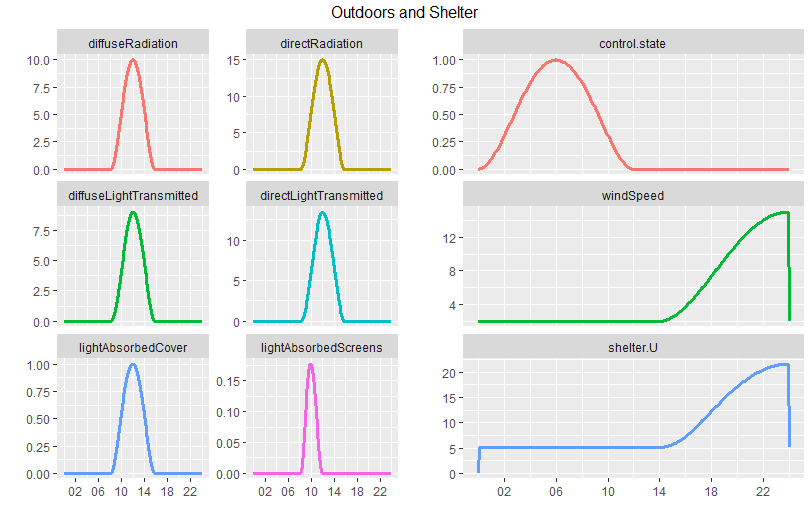
\includegraphics[width=1.0\textwidth]{graphics/vg/construction-outdoors-shelter}
\caption{Simulated outputs over \SI{24}{\hour} from the \code{outdoors} and \code{shelter} models. Produced by the \filename{vg/construction.box} script.}
\label{fig:vg-construction-outdoors-shelter}
\end{figure}

\begin{figure} [hb]
\centering
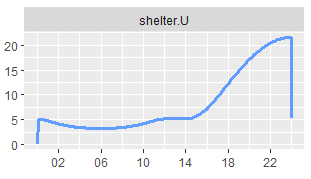
\includegraphics[width=0.5\textwidth]{graphics/vg/construction-screen-u}
\caption{Simulated shelter heat loss coefficient ($U$) over \SI{24}{\hour} when screen $U$ has been changed from $\infty$ to \SI{4}{\joule\per\meter\squared\per\kelvin}. Produced by the \filename{vg/construction-screen-u.box} script.}
\label{fig:vg-construction-screen-u}
\end{figure}
